%---------------------------------------------------------- 
% TITLE: MRes Thesis template
% AUTHOR: Andrew White 
% UNIT: FOAR705
% YEAR: Semester 2, 2019
%---------------------------------------------------------- 

%---------------------------------------------------------- 
% Personal notes:
% Before undertaking FOAR705 at Macquaire university I knew almost nothing about LaTeX, except that I had seen it mentioned before in relation to UNIX and open source software.
% This document represents over 100 hours of work on learning LaTeX, testing various options, commands, and layouts, as well as overcoming frustration when things did not work. The testing process of this document was, for the most part, a visual exercise which involved testing the pdf output and it also involved getting commands and syntax to work. I feel confident that I can use this document for my thesis and have gained enough knowledge to make changes and modify it if necessary. 
% I have formatted the document with notes and descriptions so that anyone looking at it should be able to understand what I have tried to achieve and how to make any changed that they might wish to make. I can also come back to the document at a future time and understand what I was thinking and why I did certain things. 
% For a philosophy student like myself, interested mostly in reading, writing and making arguments, this template represents a sufficient tool for writing an MRes thesis.   
%---------------------------------------------------------- 

%---------------------------------------------------------- 
% PREAMPLE
% The area between \documentclass{...} and \begin{document} is called the preamble. 
%----------------------------------------------------------

\documentclass[12pt, twoside]{book}  %% The documentclass is the first package to load in the preample. The format is \documentclass[options]{class} Between the [] we can specify a paper size and the main font size for the document, as well as if document is printed double sided. e.g. [12pt, twoside] Between the {} specifies document type e.g. article, book, report, letter, slides etc. In this particular case I will not set the paper size here, but in the geometry package below. The standard classes, article, report and book support only 3 different font sizes, 10pt, 11pt, 12pt (by default 10pt).

%---------------------------------------------------------- 
% PACKAGES
% Packages add more functions to LaTeX
%----------------------------------------------------------

\usepackage[utf8]{inputenc} %% The usepackage command is used to add more functions to LaTeX. To import a package in LaTeX, you add the \usepackage directive to the preamble of your document. The syntax is \usepackage{PACKAGENAME}. inputenc specifies the input encoding for the document, and utf8 to allows for unicode characters for use with LaTeX beyond standard ASCII. 

\renewcommand{\baselinestretch}{1.5} %% This command sets the line spacing for the document to 1.5.

\usepackage{graphicx} %% This loads the graphics function to LaTeX. The graphics function allows us to load the Macquarie University logo on the cover page. 

\graphicspath{ {images/} } %% This command tells LaTeX where to find the graphics files. In order to keep the project organised I have created a sub-folder called images where all the graphics files will to kept. 

\usepackage{marginnote} %% This loads the margin notes package.Margin notes can be added using the following syntax \marginnote{margin note text}[vertical offset, e.g 3cm]. Marginhttps://www.duplicati.com/download notes can be printed on the opposite page using \reversemarginpar right before the \marginnote{margin note text} command. We must also set the width of the margin note in the geometry package to marginparwidth=2.5cm

\usepackage[a4paper, width=150mm, top=25mm, bottom=25mm, bindingoffset=5mm, marginparwidth=2.5cm]{geometry} %% The geometry package is used to configure the page layout by entering the instructions into the square brackets. Syntax is \usepackage[INSTRUCTIONS]{geometry} The default the paper size for LaTeX is set to US letter so we need to change it to A4 paper by entering a4paper. Next we change the width of the text by entering width=150mm as well as the margin sizes at the top and bottom of the page to be 25mm using top=25mm, bottom=25mm. The option, marginparwidth=2.5cm, sets the width of the margin notes. If this is not set the margin note will go off the page. Finally, because we have specified the twoside option in the documentclass we need to set a binding offset, binding offset=6mm. On even pages the text will be slightly closer to the right side, and on odd pages it will be closer to the left. 

%% Available paper sizes include: a4paper, a5paper, b5paper, letterpaper, executivepaper, legalpaper. 

\usepackage{changepage}   % for the adjustwidth environment, which allows us to change the margins for a section of text. This is useful for large quotes. 

\usepackage{multicol} %% This package allows use the multiple column function. 

\setlength{\columnsep}{1cm} %% This command sets the space between columns to 1 cm.  

\usepackage{wrapfig} %% This package allows us to use the wrap text function to wrap around an image.

\usepackage[font=footnotesize]{caption} %% This loads the caption package and sets the size of the caption font.

%% Syntax:
%% \begin{adjustwidth}{2cm}{2cm}
%% Section of text
%% \end{adjustwidth}



%---------------------------------------------------------- 
% DOCUMENT FONTS
% This section deals with setting the font for the document.
%----------------------------------------------------------

%% The default font used for LaTeX is the Computer Modern Roman (cmr). The document is set to the default. Should you want to change the fonts, below are some options.   

    %%---- Helvetica ----
    %% \usepackage{helvet} %% This sets the Thesis document to load the helvetica packacge. 
    %% \renewcommand{\rmdefault}{phv} %%This sets the default font to phv (or helvetica)

    %%---- Latin Modern Dunhill ----
    %% \usepackage{lmodern} %% This sets the Thesis document to load the Latin Modern Dunhill packacge. 
    %% \renewcommand{\rmdefault}{lmdh} %%This sets the default font to phv (or helvetica)


%---------------------------------------------------------- 
% COLOR PACKAGE
% This section deals with loading the color package for the document.
%----------------------------------------------------------

%% This package allows us to use colour in our document. 
\usepackage[dvipsnames]{xcolor}


%---------------------------------------------------------- 
% FANCYHDR PACKAGE
% The fancyhdr package is used to set pagestyle, headers and footers.
%----------------------------------------------------------

%%------------------ FANCYHDR PACKAGE ------------------

\usepackage{fancyhdr} %% The fancyhdr package loads a special pagestyle command for headers and footers.

\pagestyle{fancy} %%  The \pproceedagestyle command changes the style of the document. The syntax is \pagestyle{option} The valid options are: plain (a plain page number), empty (Produces empty heads and feet with no page numbers), headings (Puts running headings on each page and the document style specifies what goes in the headings), myheadings (you can specify what is to go in the heading using the \markboth or thehttps://www.duplicati.com/download \markright commands), and fancy (which is a special pagestyle loaded in the the fancyhdr package which includes two custom commands, \fancyhead and \fancyfoot). 
%% The syntax for these commands is, \fancyhead[<position specifiers>]{<text>} or \fancyfoot[<position specifiers>]{<text>}. Inside the { } we put the text we want and inside t [ ] we specify where in the header we want the text to be printed. Valid options arhttps://www.duplicati.com/downloade: L = for left, R = for right, C = for centre off the header or footer and we can also specify a if this is applied to the odd (O) or even (E) pages. We can combine these, so for example, LE = left side on even pages.

\fancyhead{} %% Entering the \fancyhead{} command with a blank field clears all the header fields

\fancyhead[RO,LE]{Philosophy of work} %% This tells LaTeX we want the "Thesis title" text printed on the right-hand side of the header for the odd pages and the left for even pages.proceed

\fancyfoot{} %% Entering the \fancyfoot{} command with a blank field clears the footer fields.

\fancyfoot[LE,RO]{\thepage} %% The LE and RO options makes the page number appear on the left side of the footer for an even pages and the right side for an odd pages. The \thepage command returns the page number of the page it's used on.


\fancyfoot[LO,CE]{\ifnum \value{chapter}>0 Chapter \thechapter\fi} %% This prints the chapter on the left side on odd pages and the centre on even pages. 

\fancyfoot[CO,RE]{Andrew white} %% This prints the text specified in {Author Name} in the centre on odd pages anlatex thesis d the right on even pages. 

% The \renewcommand is used to redefine a command. The syntax is \renewcommand{cmd}[args]{def}.

\renewcommand{\headrulewidth}{0.2pt} %% Here we use the \renewcommand to change the thickness of the lines in the headers to 0.4pt. This is thinner than the default.

\renewcommand{\footrulewidth}{0.2pt} %% Here we use the \renewcommand to change the thickness of the lines in the footer to 0.4pt.

%---------------------------------------------------------- 
% BIBLIOGRAPHY
% This section sets the biblatex bibliography package.
%----------------------------------------------------------

%% The bibliography information is contained within the file bibliography.bib. Refer to this file for detailed information regarding the syntax of the bibliography entries. 

%% To make citations we can use the cite command. The Syntax is \cite{citation key}. We can also use the \parencite{citation key} command which prints citations in parentheses. However, it prints the citation in square brackets when using the numeric or alphabetic referencing styles. 

\usepackage[backend=biber,style=authoryear,sorting=nyt]{biblatex} %% -- This command loads the biblatex bibliography package and calls the alphabetic style bibliography. If we omit the square brackets the bibliography will print the default style citations which is the numeric style. 
%% OPTIONS: [style=authoryear,sorting=none] for authoryear style with no sorting, or [style=authoryear,sorting=ynt] for authoryear style with sorting for year, name, title.  [style=alphabetic]{biblatex} for alphabetic style.  
%% In this template I have selected the Name, Year, Title sorting. [style=authoryear,sorting=nyt] 
\addbibresource{references.bib} %% This command loads the  bibliography.bib file. 

%---------------------------------------------------------- 
% CITATION INFORMATION
% Notes on citations
%----------------------------------------------------------

%% To add these extra notes to citations we use two sets of square brackets in the citation command before the curly brackets. These are the postnote and the prenote.

%% Examples of Syntax: 
%% \parencite[prenote][postnote]{citation key}
%% \cite[][]{citation key}
%% If we only include one set of square brackets, e.g. \parencite[p.22]{citation key} it will assume the contents of the brackets is a postnote. 
%% If we want a prenote we need open the second set of square brackets and leave it empty. e.g. Here are some examples: \parencite[see][]{citation key}

%% For more information on referencing refer to the online biblatex guide, http://mirror.aarnet.edu.au/pub/CTAN/macros/latex/contrib/biblatex/doc/biblatex.pdf


%---------------------------------------------------------- 
% TITLE PAGE
% Notes on citations
%----------------------------------------------------------


%% The following lines in the preamble defines the information to be included on the title page. \title {} prints the title of the document. Inside the outer curly brackets of the \title we have a subheading and an image. \large prints a subheading in large text (this is large text, but smaller than the title text) \includegraphies the logo graphics to be printed on the cover page. The location of images was previously set to the images/ folder using the \graphicspath command. 

% This code is redundant since I have decided to load the title page from a separate file. It is left here as a reference in case I decide not to use the separate titlepage file at a later date.

\title{{Philosophy of Work}\\ 
{\large MRes Thesis Template}\\
{
\includegraphics{MQ_INT_VER_RGB_POS.PNG}}
}
\author{Andrew White} %% Name of author to be printed on the cover page.
\date{October 2019} %% Date to be printed on the cover page.

%---------------------------------------------------------- 
% START OF LATEX DOCUMENT
% This is the beginning of the document proper
%----------------------------------------------------------

\begin{document} %% The area between \begin{document} and \end{document} is the main text of the document. 

\frontmatter % Enter after the (\begin{document}) to switch page numbering to Roman numerals 

%% \maketitle %% This is used to make a title from the information above. However, the %-------------------------------------------------
% TITLE PAGE
% This is a separate document for the titlepage, which is loaded into the main document.
%-------------------------------------------------

%% The following lines define the information to be included on the title page. \title {} prints the title of the document. Inside the outer curly brackets of the \title we have a subheading and an image. \large prints a subheading in large text (this is large text, but smaller than the title text) \includegraphies the logo graphics to be printed on the cover page. The location of images was previously set to the images/ folder using the \graphicspath command. 

\begin{titlepage} %% Begin this document called titlepage
   \begin{center} %% This encloses everything on the titlepage to be centred. 
       \vspace*{1cm} %% This is the gap between the top of the page and the first line of text. 
 
        \Huge %% sets the size of the title text to Huge (for details about changing font types and sizes refer to chapter 02 
        \textbf{Philosophy of Work} %% This is the thesis title
        
        \hrulefill %% This puts a horizontal line under the heading of the thesis.
 
        \Large %% sets the size of the subtitle to LARGE
        
        \vspace{0.5cm} %% this sets the space between the heading and the subtitle
        MRes Thesis Template
 
        \vspace{1.3cm} %% this sets the space between the subtitle and the Author's name
 
        \LARGE
 
        \textbf{Andrew White}
 
        \vfill %% The \vfill command will automatically add in enough vertical space to fill the page.
 
        \Large %% sets the size to Large
 
       A thesis presented for the degree of\\
       Masters of Research in Philosophy
 
       \vspace{1cm}
 
       
\includegraphics[width=0.5\textwidth]{MQ_INT_VER_RGB_POS.PNG} %% The \includegraphics command loads the graphics file MQ_INT_VER_RGB_POS.PNG. The width=0.5\textwidth tells LaTeX to set the width of the graphics file to be 0.5 of the width of the text.  
 
    \large  %% sets the size of the subtitle to Large
       Department of Philosophy\\
       Macquarie University\\
       Sydney, Australia\\
       October 2019
 
   \end{center} %% This ends the \begin{center} environment.
\end{titlepage} %% End this document called titlepage
 command will call the titlepage from a separate file called titlepage.tex

%-------------------------------------------------
% TITLE PAGE
% This is a separate document for the titlepage, which is loaded into the main document.
%-------------------------------------------------

%% The following lines define the information to be included on the title page. \title {} prints the title of the document. Inside the outer curly brackets of the \title we have a subheading and an image. \large prints a subheading in large text (this is large text, but smaller than the title text) \includegraphies the logo graphics to be printed on the cover page. The location of images was previously set to the images/ folder using the \graphicspath command. 

\begin{titlepage} %% Begin this document called titlepage
   \begin{center} %% This encloses everything on the titlepage to be centred. 
       \vspace*{1cm} %% This is the gap between the top of the page and the first line of text. 
 
        \Huge %% sets the size of the title text to Huge (for details about changing font types and sizes refer to chapter 02 
        \textbf{Philosophy of Work} %% This is the thesis title
        
        \hrulefill %% This puts a horizontal line under the heading of the thesis.
 
        \Large %% sets the size of the subtitle to LARGE
        
        \vspace{0.5cm} %% this sets the space between the heading and the subtitle
        MRes Thesis Template
 
        \vspace{1.3cm} %% this sets the space between the subtitle and the Author's name
 
        \LARGE
 
        \textbf{Andrew White}
 
        \vfill %% The \vfill command will automatically add in enough vertical space to fill the page.
 
        \Large %% sets the size to Large
 
       A thesis presented for the degree of\\
       Masters of Research in Philosophy
 
       \vspace{1cm}
 
       
\includegraphics[width=0.5\textwidth]{MQ_INT_VER_RGB_POS.PNG} %% The \includegraphics command loads the graphics file MQ_INT_VER_RGB_POS.PNG. The width=0.5\textwidth tells LaTeX to set the width of the graphics file to be 0.5 of the width of the text.  
 
    \large  %% sets the size of the subtitle to Large
       Department of Philosophy\\
       Macquarie University\\
       Sydney, Australia\\
       October 2019
 
   \end{center} %% This ends the \begin{center} environment.
\end{titlepage} %% End this document called titlepage
 %%Loads the title page from the file titlepage.tex

%% In order to keep the project organized and manageable I have created a sub-folder called chapters. Inside this folder there are .tex files for each chapter of the thesis as well as an appendix. The \input{} command loads the tex file into the main document. For example, %-------------------------------------------------
% CHAPTER 2
% This is a separate document for the Chapter 2, which is loaded into the main document.
%-------------------------------------------------

%% Chapter 02 will layout standard guidelines for font types and sizes 
%% The following are the available font sizes ranging from smallest to largest.



\section{Introduction}

This chapter gives some examples of how to change font sizes, families, styles and colors. Font size  commands change to size of the font. Font families change the typeface of the font. By default, LaTeX is set to the serif typeface (a.k.a. roman). Font styles refer to such things as bold, italics and underlined. Colours can be adjusted for the font, the font background and the page colour. 


\section{Font Sizes}

Font sizes are identified by special tags or commands, the actual size is not absolute but relative to the font size declared in the documentclass statement found at the start of the main.tex file.

\vspace{0.3cm}

\underline{This is a list of special tags for changing the font size}
\begin{verbatim}
\tiny 
\scriptsize
\footnotesize
\small
\normalsize
\large
\Large
\LARGE
\huge
\Huge
\end{verbatim}



If we use a set of curly brackets after the font tag, for example, \verb|\Large{text}| then only the text inside the brackets will be affected by the font tag command. In this sentence the {\huge huge font size} is set within the curly brackets \verb|{}| and then we can change to the {\footnotesize Foot note size font at the end of the sentence}. When we resume typing the font size will be back to normal because we set the huge font and footnote font inside the curly brackets. 

\vspace{0.3cm}

If we write the font tag without curly brackets, then the size that we set will become the default size from that point onward unless it is changed. For example, in the next sentence I will use the \verb|\footnotesize| font spacial tag. \footnotesize This font is written in footnotesize font without curly brackets. 

\vspace{0.4cm}

If I create a new paragraph the font size will still be set the footnotesize. In order to change the font size back we need to issue the \verb|\normalsize| font special tag. \normalsize This font is now set back to normal size.     

\vspace{0.4cm}

Next I will give examples of each of the font sizes. 

\vspace{0.4cm}


The following text is written in the {\tiny tiny font size.} 

The following text is written in the {\scriptsize scriptsize font size.} 

The following text is written in the {\footnotesize footnotesize font size.} 

The following text is written in the {\small small font size.} 

The following text is written in the {\normalsize normal font size.} 

The following text is written in the {\large large font size.} 

The following text is written in the {\Large Large font size.} Note the difference between large and Large with the use of the capital L for the larger version. 

The following text is written in the {\LARGE LARGE font size.} Note again the font size LARGE has all capital letters.

The following text is written in the {\huge huge font size.} 

The following text is written in the {\Huge Huge font size.} Again, note the difference between huge and Huge Large with the use of the capital H for the larger version. 

\newpage

\section{Font Families}

Font families change the typeface of the font. By default, LaTeX is set to the serif typeface (a.k.a. roman). There are other typefaces such as sans serif and typewriter.

{\fontfamily{qcr}\selectfont This text uses Gyre Cursor font typeface}

{\fontfamily{ptm}\selectfont This text uses the times font typeface}

{\fontfamily{put}\selectfont This text uses the utopia / fourier font typeface}

{\fontfamily{pcr}\selectfont This text uses the courier font typeface}

 {\fontfamily{cmss}\selectfont This text uses the Computer Modern Sans Serif font typeface}

\newpage

\section{Font Styles}

Font styles generally refer to such elements as bold, italics and underlined, however, there are other styles which can be set. The following table shows the available options.

\begin{figure}[h]
\centering
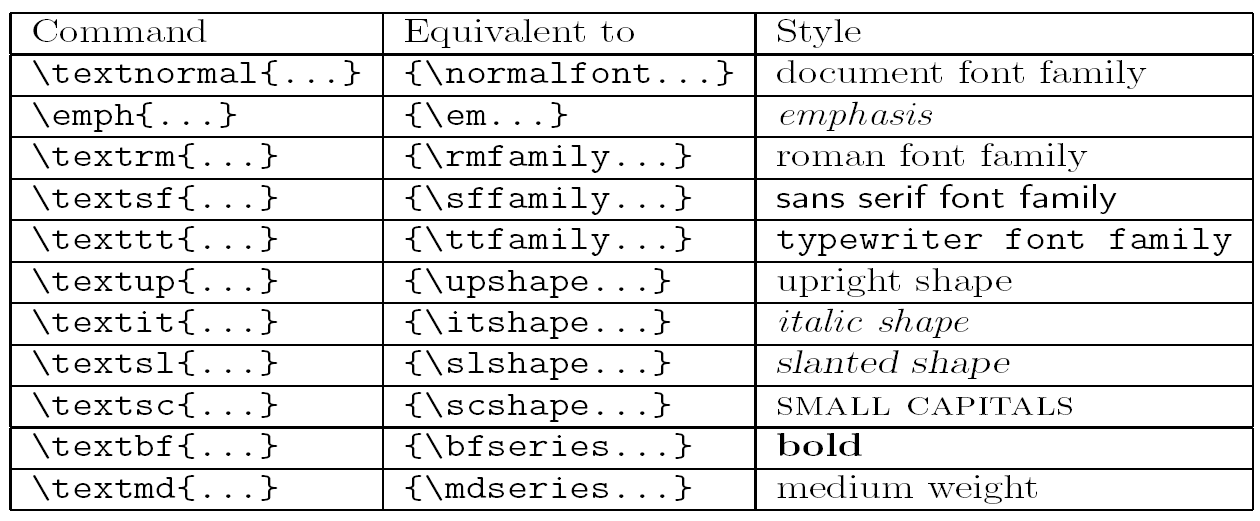
\includegraphics[width=0.7\textwidth]{images/Latex_styles_table.png}
\caption{Available Font styles}
\label{fig:x Available Font styles} \parencite{wiki:003}
\end{figure}



\begin{adjustwidth}{2cm}{2cm}

Examples:

\textsf{This text is written in the sans serif font family}

\textnormal{This text is written in the normal document font family}

\texttt{This text is written in the typewriter family}

We can write some \textbf{bold text}

\textsc{we can write a sentence in small capitals.} 

We can write text with an \emph{emphasis}

We can write text with an \textit{italics}

\end{adjustwidth}

\vspace{0.4cm}

The emphasis command might seem like it is the same thing as italic but it does behave slightly differently. 

If we type a sentence in normal text the \emph{emphasis} will appear like italics.

\textit{If we type a sentence in in italics the  \emph{emphasis} will appear normally creating an emphasis.}

\newpage

\section{Font Colours}

In order to use colours in LaTeX we need to ad the \verb|\usepackage{xcolor}| command to the preample in the main.tex file. 

dvipsnames Makes the colour names for the driver dvips available. From this new set of colour names, the example uses: ForestGreen, RubineRed and BurntOrange. See the reference guide for a complete list of possible colours.

There are two very useful commands. 

\verb|\textcolor{color}{text}| and, 

\verb|\colorbox{color}{text}|

\textcolor{blue}{This is an example of blue text}

\colorbox{BurntOrange}{This is an example of a colorbox in BurntOrange}

\textcolor{red}{This whole paragraph is in red text. Curabitur ac augue sit amet enim pretium semper. Ut at finibus ligula. In hac habitasse platea dictumst. Duis porta felis lectus, non sollicitudin turpis ultricies in. Duis tristique justo feugiat elit sollicitudin, at efficitur sapien mollis. Etiam sem nisi, hendrerit vel bibendum non, vehicula vitae nibh.}

\vspace{0.4cm}

\begin{figure}[h]
\centering
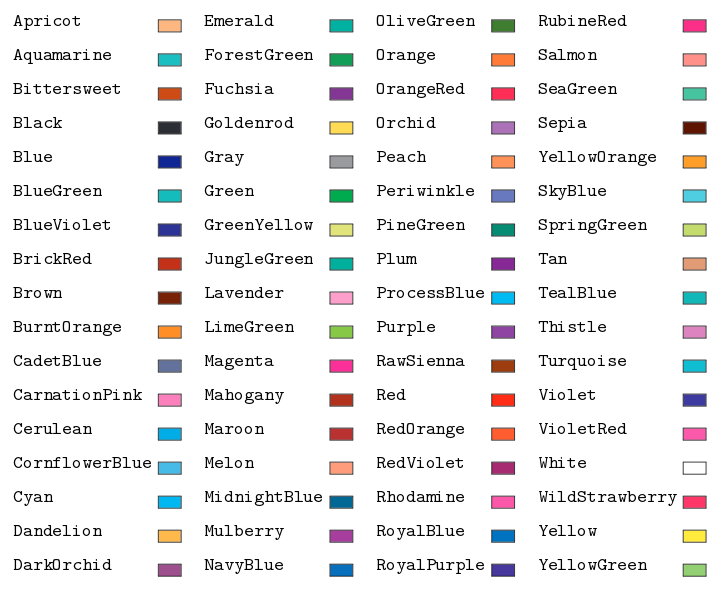
\includegraphics[width=0.7\textwidth]{images/ColoursEx6.png}
\caption{Colour names available with the dvipsnames option}
\label{fig:x Color options} \parencite{overleaf01}
\end{figure}


\newpage

\pagecolor{black}
\color{white}

\section{Page and Font Colours}


It is possible using the \verb|pagecolor{}| \verb|color{}| commands to change to color of a page and font. This page is set to BLACK and the text is set to WHITE.

\vspace{0.4cm}

Lorem ipsum dolor sit amet, consectetur adipiscing elit. Nam rutrum magna ut mi sollicitudin pellentesque. Vivamus sit amet euismod nibh. Sed ornare enim vel tellus faucibus egestas. Donec sit amet diam placerat, interdum sapien sit amet, pulvinar neque. Morbi eget massa ut erat vehicula efficitur. Aenean vitae luctus magna. Nam varius ligula nec nunc egestas ultricies. Quisque vel vehicula mauris. Phasellus venenatis tortor et lorem aliquam luctus.


\textcolor{red}{Lorem ipsum dolor sit amet, consectetur adipiscing elit. Nam rutrum magna ut mi sollicitudin pellentesque. Vivamus sit amet euismod nibh. Sed ornare enim vel tellus faucibus egestas. Donec sit amet diam placerat, interdum sapien sit amet, pulvinar neque. Morbi eget massa ut erat vehicula efficitur. Aenean vitae luctus magna. Nam varius ligula nec nunc egestas ultricies. Quisque vel vehicula mauris. Phasellus venenatis tortor et lorem aliquam luctus.}


Lorem ipsum dolor sit amet, consectetur adipiscing elit. Nam rutrum magna ut mi sollicitudin pellentesque. Vivamus sit amet euismod nibh. Sed ornare enim vel tellus faucibus egestas. Donec sit amet diam placerat, interdum sapien sit amet, pulvinar neque. Morbi eget massa ut erat vehicula efficitur. Aenean vitae luctus magna. Nam varius ligula nec nunc egestas ultricies. Quisque vel vehicula mauris. Phasellus venenatis tortor et lorem aliquam luctus.

\textbf{Lorem ipsum dolor sit amet, consectetur adipiscing elit. Nam rutrum magna ut mi sollicitudin pellentesque. Vivamus sit amet euismod nibh. Sed ornare enim vel tellus faucibus egestas. Donec sit amet diam placerat, interdum sapien sit amet, pulvinar neque. Morbi eget massa ut erat vehicula efficitur. Aenean vitae luctus magna.}


\newpage

\pagecolor{white}

\color{black}

To reset the page and font colors we re-issue the commands \verb|pagecolor{}| and  \verb|color{}| with page colour set back to white and text set to black. 

\vspace{0.4cm}

Lorem ipsum dolor sit amet, consectetur adipiscing elit. Nam rutrum magna ut mi sollicitudin pellentesque. Vivamus sit amet euismod nibh. Sed ornare enim vel tellus faucibus egestas. Donec sit amet diam placerat, interdum sapien sit amet, pulvinar neque. Morbi eget massa ut erat vehicula efficitur. Aenean vitae luctus magna. Nam varius ligula nec nunc egestas ultricies. Quisque vel vehicula mauris. Phasellus venenatis tortor et lorem aliquam luctus.


Lorem ipsum dolor sit amet, consectetur adipiscing elit. Nam rutrum magna ut mi sollicitudin pellentesque. Vivamus sit amet euismod nibh. Sed ornare enim vel tellus faucibus egestas. Donec sit amet diam placerat, interdum sapien sit amet, pulvinar neque. Morbi eget massa ut erat vehicula efficitur. Aenean vitae luctus magna. Nam varius ligula nec nunc egestas ultricies. Quisque vel vehicula mauris. Phasellus venenatis tortor et lorem aliquam luctus.


Lorem ipsum dolor sit amet, consectetur adipiscing elit. Nam rutrum magna ut mi sollicitudin pellentesque. Vivamus sit amet euismod nibh. Sed ornare enim vel tellus faucibus egestas. Donec sit amet diam placerat, interdum sapien sit amet, pulvinar neque. Morbi eget massa ut erat vehicula efficitur. Aenean vitae luctus magna. Nam varius ligula nec nunc egestas ultricies. Quisque vel vehicula mauris. Phasellus venenatis tortor et lorem aliquam luctus.



Lorem ipsum dolor sit amet, consectetur adipiscing elit. Nam rutrum magna ut mi sollicitudin pellentesque. Vivamus sit amet euismod nibh. Sed ornare enim vel tellus faucibus egestas. Donec sit amet diam placerat, interdum sapien sit amet, pulvinar neque. Morbi eget massa ut erat vehicula efficitur. Aenean vitae luctus magna. Nam varius ligula nec nunc egestas ultricies. Quisque vel vehicula mauris. Phasellus venenatis tortor et lorem aliquam luctus.Lorem ipsum dolor sit amet, consectetur adipiscing elit. Nam rutrum magna ut mi sollicitudin pellentesque. Vivamus sit amet euismod nibh. Sed ornare enim vel tellus faucibus egestas. Donec sit amet diam placerat, interdum sapien sit amet, pulvinar neque. Morbi eget massa ut erat vehicula efficitur. Aenean vitae luctus magna. Nam varius ligula nec nunc egestas ultricies. Quisque vel vehicula mauris. Phasellus venenatis tortor et lorem aliquam luctus.


Lorem ipsum dolor sit amet, consectetur adipiscing elit. Nam rutrum magna ut mi sollicitudin pellentesque. Vivamus sit amet euismod nibh. Sed ornare enim vel tellus faucibus egestas. Donec sit amet diam placerat, interdum sapien sit amet, pulvinar neque. Morbi eget massa ut erat vehicula efficitur. Aenean vitae luctus magna. Nam varius ligula nec nunc egestas ultricies. Quisque vel vehicula mauris. Phasellus venenatis tortor et lorem aliquam luctus.


\newpage
 loads the file chapter02.tex from the directory chapters. It is important that this directory structure is maintained otherwise LaTeX will not know where to find the chapters and appendix. 

\tableofcontents

%% Abstract, dedication, declaration and acknowledgements. To setup up our document so that the the abstract, dedication, declaration and acknowledgements are not numbered (unnumbered chapters) or included in Contents we use the \chapter command and add an asterisk. e.g \chapter*{Abstract}.. 

\listoffigures 

%%------------------ ABSTRACT ------------------
\newpage

%-------------------------------------------------
% ABSTRACT
% This is a separate document for the Abstract, which is loaded into the main document.
%-------------------------------------------------

\thispagestyle{plain} %% This changes the page style to plain to stop the headers being added in
\begin{center} %% This encloses everything on the abstract to be centred.
    \Large 
    \textbf{Philosophy of Work}
 
    \vspace{0.5cm} %% This is the gap of 0.5cm between the title of the abstract and subtitle. 
    \large
    MRes Thesis Template
 
    \vspace{0.5cm} %% This is the gap of 0.5cm between the subtitle of the abstract and authors name. 
    \textbf{Andrew White}
 
    \vspace{0.9cm}
    \textbf{Abstract}
\end{center}
Lorem ipsum dolor sit amet, consectetur adipiscing elit. Nam rutrum magna ut mi sollicitudin pellentesque. Vivamus sit amet euismod nibh. Sed ornare enim vel tellus faucibus egestas. Donec sit amet diam placerat, interdum sapien sit amet, pulvinar neque. Morbi eget massa ut erat vehicula efficitur. Aenean vitae luctus magna. Nam varius ligula nec nunc egestas ultricies. Quisque vel vehicula mauris. Phasellus venenatis tortor et lorem aliquam luctus.

Quisque blandit nulla et velit auctor, a interdum ex imperdiet. Cras eget quam velit. Sed vel ante felis. Phasellus dictum lectus ac metus ornare facilisis. Aliquam placerat diam id viverra aliquam. Curabitur elit nulla, lacinia id euismod eu, elementum ullamcorper felis. Sed ut magna sit amet orci iaculis aliquet. Nulla facilisi. Sed elit nunc, posuere quis lorem a, vestibulum bibendum libero. Pellentesque ultricies est ut nisi finibus, ac commodo augue dictum. Vivamus laoreet sagittis placerat.

Curabitur ac augue sit amet enim pretium semper. Ut at finibus ligula. In hac habitasse platea dictumst. Duis porta felis lectus, non sollicitudin turpis ultricies in. Duis tristique justo feugiat elit sollicitudin, at efficitur sapien mollis. Etiam sem nisi, hendrerit vel bibendum non, vehicula vitae nibh. Aliquam commodo metus a dolor dignissim, sed lobortis nisl finibus. Fusce finibus, nibh et vehicula malesuada, diam massa semper ipsum, et volutpat lorem ipsum venenatis sapien. Quisque ac turpis tincidunt tortor vestibulum semper vel at magna. Nam erat nulla, egestas ac fringilla vehicula, tempor a velit. Donec ipsum velit, porta nec iaculis ac, sollicitudin nec magna. Nullam pretium mauris et nulla fringilla, at vulputate tellus vulputate. Fusce venenatis nisi quis vestibulum facilisis. Suspendisse enim orci, blandit quis elementum ut, tincidunt id nisl.
 %% this loads the abstract from a separate file called abstract.tex 


%%------------------ DEDICATION ------------------
 
\chapter*{Dedication}
This is the dedication page

%%------------------ DECLARATION ------------------
 
\chapter*{Declaration}
I declare that...

%%------------------ ACKNOWLEDGEMENTS ------------------
 
\chapter*{Acknowledgements}
I want to thank...

%---------------------------------------------------------- 
% THE MAIN THESIS TEXT BEGINS HERE
% This is the beginning of the document text
%----------------------------------------------------------

\mainmatter % Enter right before the first chapter of the book to turn the numbering to arabic page numbering and restarts the page counter. 

\chapter{Introduction}
LaTeX is a document preparation system. This means LaTeX uses markup tagging commands to structure and stylise a document, to add citations, margin notes, footnotes etc. And it uses plain text for the content which is then generated into a Portable Document Format (PDF) file. 

In this introductory chapter I will setup a template of how to do citations, footnotes and margin notes. The text in the document is generic and only instrumental for the purposes of demonstration, with some explanatory notes. Please refer to the LaTeX files for a more in depth description of the document structure and command syntax. 

\vspace{0.5cm}

\section{In-text Citations}

Lorem ipsum  \parencite{sennett1998corrosion} dolor sit amet, consectetur adipiscing elit. Nam rutrum magna ut mi sollicitudin pellentesque. Vivamus sit amet euismod nibh. Sed ornare enim vel tellus faucibus egestas. Donec sit amet diam placerat, interdum sapien sit amet, pulvinar neque. Morbi eget massa ut erat vehicula efficitur. Aenean vitae luctus magna. Nam varius ligula nec nunc egestas ultricies. Quisque vel vehicula mauris. Phasellus venenatis tortor et lorem aliquam luctus.\footnote{First example footnote text}

Cras eget quam velit. Sed vel ante felis. Phasellus dictum lectus ac metus ornare facilisis. Aliquam placerat diam id  aliquam. Curabitur elit nulla, lacinia id euismod eu, elementum ullamcorper felis. Sed ut magna sit amet orci iaculis aliquet.  \footnote{This is the second example footnote text to test layout}

Curabitur ac augue sit amet enim pretium semper. \marginnote{This is an example of a margin note.}  Ut at finibus ligula. In hac habitasse platea dictumst. Duis porta felis lectus, non sollicitudin turpis ultricies in. Duis tristique justo feugiat elit sollicitudin, at efficitur sapien mollis. Etiam sem nisi, hendrerit vel bibendum non, vehicula vitae nibh. Aliquam commodo metus a dolor dignissim, sed lobortis nisl finibus. 

Vestibulum ligula sem, volutpat eu erat. Nulla interdum risus non metus vehicula. Sed ligula ante, ullamcorper egestas ex. Nunc tincidunt rhoncus neque, ac luctus ligula interdum nec. Interdum et malesuada fames ac ante ipsum primis in faucibus.\parencite[see][p.10]{mcguigan2014neoliberal}

 Maecenas ac dictum sapien. Integer id dui vel augue luctus egestas non quis purus. Nam quis, gravida lacus vitae, egestas magna. Proin ultrices quis tellus id ornare. Nulla ut pulvinar tellus. Mauris laoreet suscipit nisl, euismod vestibulum nisi. Proin vel mauris non sapien bibendum fringilla. \parencite[see][]{Han2015WhyRevolution}

%% =======Citation Guide=======

%% See main.text CITATION GUIDE for information of making citations. 

\section{Extended Text Citations}

In this section I will demonstrate the difference between the quote and the adjustwidth options for an extended text quotation. 

\vspace{0.4cm}

This first example uses the \verb|\begin{quote}| option and the text size \verb|\small{}|. 

\vspace{0.4cm}

Lorem ipsum dolor sit amet, consectetur adipiscing elit. Nam rutrum magna ut mi sollicitudin pellentesque. Vivamus sit amet euismod nibh. Sed ornare enim vel tellus faucibus egestas. Donec sit amet diam placerat, interdum sapien sit amet, pulvinar neque. Morbi eget massa ut erat vehicula efficitur. 

\begin{quote}

\small{This section of text is an extended quote. Quisque blandit nulla et velit auctor, a interdum ex imperdiet. Cras eget quam velit. Sed vel ante felis. Phasellus dictum lectus ac metus ornare facilisis. Aliquam placerat diam id viverra aliquam. Curabitur elit nulla, lacinia id euismod eu, elementum ullamcorper felis.} \parencite[][p. 100]{sennett1998corrosion}

\end{quote}

Lorem ipsum dolor sit amet, consectetur adipiscing elit. Nam rutrum magna ut mi sollicitudin pellentesque. Vivamus sit amet euismod nibh. Sed ornare enim vel tellus faucibus egestas. Donec sit amet diam placerat, interdum sapien sit amet, pulvinar neque. Morbi eget massa ut erat vehicula efficitur. 

\newpage

This second example uses the \verb|\begin{adjustwidth}{2cm}{2cm}| option and the text size \verb|\small{}|. Here we can adjust the desired margins for the quotation. 

\vspace{0.4cm}

Lorem ipsum dolor sit amet, consectetur adipiscing elit. Nam rutrum magna ut mi sollicitudin pellentesque. Vivamus sit amet euismod nibh. Sed ornare enim vel tellus faucibus egestas. Donec sit amet diam placerat, interdum sapien sit amet, pulvinar neque. Morbi eget massa ut erat vehicula efficitur. 

\begin{adjustwidth}{2cm}{2cm}

\small{This section of text is an extended quote. Quisque blandit nulla et velit auctor, a interdum ex imperdiet. Cras eget quam velit. Sed vel ante felis. Phasellus dictum lectus ac metus ornare facilisis. Aliquam placerat diam id viverra aliquam. Curabitur elit nulla, lacinia id euismod eu, elementum ullamcorper felis.} \parencite[][p. 100]{sennett1998corrosion}

\end{adjustwidth}

Curabitur ac augue sit amet enim pretium semper. Ut at finibus ligula. In hac habitasse platea dictumst. Duis porta felis lectus, non sollicitudin turpis ultricies in. Duis tristique justo feugiat elit sollicitudin, at efficitur sapien mollis. Etiam sem nisi, hendrerit vel bibendum non, vehicula vitae nibh. Aliquam commodo metus a dolor dignissim, sed lobortis nisl finibus. 
 %% This loads the introduction.tex file from the chapters sub directory. The introduction contains same example footnotes. margin notes and citations.  Footnotes are included in the text using this syntax \footnote{example footnote text}. 
 
\chapter{Fonts}
%-------------------------------------------------
% CHAPTER 2
% This is a separate document for the Chapter 2, which is loaded into the main document.
%-------------------------------------------------

%% Chapter 02 will layout standard guidelines for font types and sizes 
%% The following are the available font sizes ranging from smallest to largest.



\section{Introduction}

This chapter gives some examples of how to change font sizes, families, styles and colors. Font size  commands change to size of the font. Font families change the typeface of the font. By default, LaTeX is set to the serif typeface (a.k.a. roman). Font styles refer to such things as bold, italics and underlined. Colours can be adjusted for the font, the font background and the page colour. 


\section{Font Sizes}

Font sizes are identified by special tags or commands, the actual size is not absolute but relative to the font size declared in the documentclass statement found at the start of the main.tex file.

\vspace{0.3cm}

\underline{This is a list of special tags for changing the font size}
\begin{verbatim}
\tiny 
\scriptsize
\footnotesize
\small
\normalsize
\large
\Large
\LARGE
\huge
\Huge
\end{verbatim}



If we use a set of curly brackets after the font tag, for example, \verb|\Large{text}| then only the text inside the brackets will be affected by the font tag command. In this sentence the {\huge huge font size} is set within the curly brackets \verb|{}| and then we can change to the {\footnotesize Foot note size font at the end of the sentence}. When we resume typing the font size will be back to normal because we set the huge font and footnote font inside the curly brackets. 

\vspace{0.3cm}

If we write the font tag without curly brackets, then the size that we set will become the default size from that point onward unless it is changed. For example, in the next sentence I will use the \verb|\footnotesize| font spacial tag. \footnotesize This font is written in footnotesize font without curly brackets. 

\vspace{0.4cm}

If I create a new paragraph the font size will still be set the footnotesize. In order to change the font size back we need to issue the \verb|\normalsize| font special tag. \normalsize This font is now set back to normal size.     

\vspace{0.4cm}

Next I will give examples of each of the font sizes. 

\vspace{0.4cm}


The following text is written in the {\tiny tiny font size.} 

The following text is written in the {\scriptsize scriptsize font size.} 

The following text is written in the {\footnotesize footnotesize font size.} 

The following text is written in the {\small small font size.} 

The following text is written in the {\normalsize normal font size.} 

The following text is written in the {\large large font size.} 

The following text is written in the {\Large Large font size.} Note the difference between large and Large with the use of the capital L for the larger version. 

The following text is written in the {\LARGE LARGE font size.} Note again the font size LARGE has all capital letters.

The following text is written in the {\huge huge font size.} 

The following text is written in the {\Huge Huge font size.} Again, note the difference between huge and Huge Large with the use of the capital H for the larger version. 

\newpage

\section{Font Families}

Font families change the typeface of the font. By default, LaTeX is set to the serif typeface (a.k.a. roman). There are other typefaces such as sans serif and typewriter.

{\fontfamily{qcr}\selectfont This text uses Gyre Cursor font typeface}

{\fontfamily{ptm}\selectfont This text uses the times font typeface}

{\fontfamily{put}\selectfont This text uses the utopia / fourier font typeface}

{\fontfamily{pcr}\selectfont This text uses the courier font typeface}

 {\fontfamily{cmss}\selectfont This text uses the Computer Modern Sans Serif font typeface}

\newpage

\section{Font Styles}

Font styles generally refer to such elements as bold, italics and underlined, however, there are other styles which can be set. The following table shows the available options.

\begin{figure}[h]
\centering
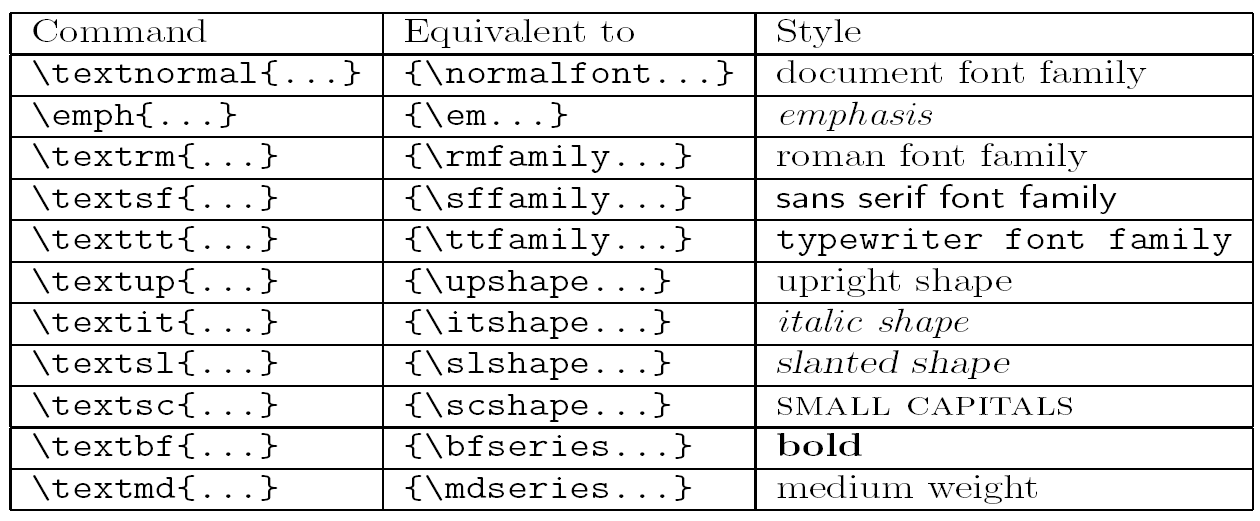
\includegraphics[width=0.7\textwidth]{images/Latex_styles_table.png}
\caption{Available Font styles}
\label{fig:x Available Font styles} \parencite{wiki:003}
\end{figure}



\begin{adjustwidth}{2cm}{2cm}

Examples:

\textsf{This text is written in the sans serif font family}

\textnormal{This text is written in the normal document font family}

\texttt{This text is written in the typewriter family}

We can write some \textbf{bold text}

\textsc{we can write a sentence in small capitals.} 

We can write text with an \emph{emphasis}

We can write text with an \textit{italics}

\end{adjustwidth}

\vspace{0.4cm}

The emphasis command might seem like it is the same thing as italic but it does behave slightly differently. 

If we type a sentence in normal text the \emph{emphasis} will appear like italics.

\textit{If we type a sentence in in italics the  \emph{emphasis} will appear normally creating an emphasis.}

\newpage

\section{Font Colours}

In order to use colours in LaTeX we need to ad the \verb|\usepackage{xcolor}| command to the preample in the main.tex file. 

dvipsnames Makes the colour names for the driver dvips available. From this new set of colour names, the example uses: ForestGreen, RubineRed and BurntOrange. See the reference guide for a complete list of possible colours.

There are two very useful commands. 

\verb|\textcolor{color}{text}| and, 

\verb|\colorbox{color}{text}|

\textcolor{blue}{This is an example of blue text}

\colorbox{BurntOrange}{This is an example of a colorbox in BurntOrange}

\textcolor{red}{This whole paragraph is in red text. Curabitur ac augue sit amet enim pretium semper. Ut at finibus ligula. In hac habitasse platea dictumst. Duis porta felis lectus, non sollicitudin turpis ultricies in. Duis tristique justo feugiat elit sollicitudin, at efficitur sapien mollis. Etiam sem nisi, hendrerit vel bibendum non, vehicula vitae nibh.}

\vspace{0.4cm}

\begin{figure}[h]
\centering
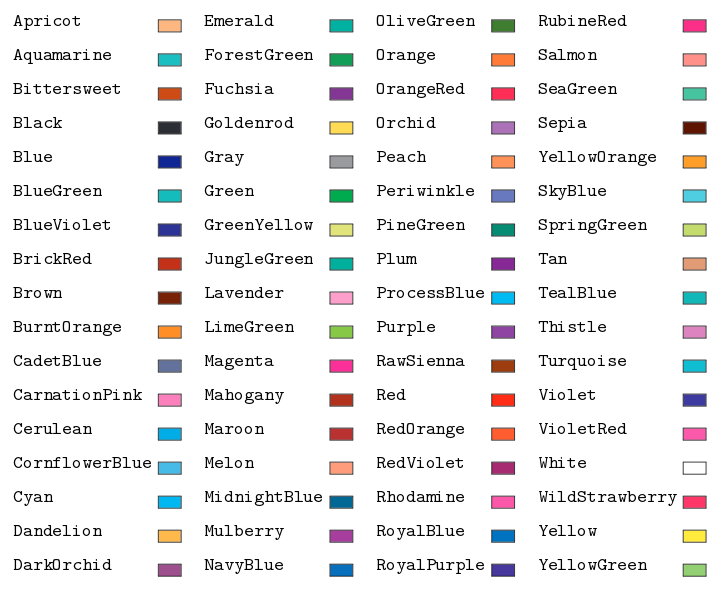
\includegraphics[width=0.7\textwidth]{images/ColoursEx6.png}
\caption{Colour names available with the dvipsnames option}
\label{fig:x Color options} \parencite{overleaf01}
\end{figure}


\newpage

\pagecolor{black}
\color{white}

\section{Page and Font Colours}


It is possible using the \verb|pagecolor{}| \verb|color{}| commands to change to color of a page and font. This page is set to BLACK and the text is set to WHITE.

\vspace{0.4cm}

Lorem ipsum dolor sit amet, consectetur adipiscing elit. Nam rutrum magna ut mi sollicitudin pellentesque. Vivamus sit amet euismod nibh. Sed ornare enim vel tellus faucibus egestas. Donec sit amet diam placerat, interdum sapien sit amet, pulvinar neque. Morbi eget massa ut erat vehicula efficitur. Aenean vitae luctus magna. Nam varius ligula nec nunc egestas ultricies. Quisque vel vehicula mauris. Phasellus venenatis tortor et lorem aliquam luctus.


\textcolor{red}{Lorem ipsum dolor sit amet, consectetur adipiscing elit. Nam rutrum magna ut mi sollicitudin pellentesque. Vivamus sit amet euismod nibh. Sed ornare enim vel tellus faucibus egestas. Donec sit amet diam placerat, interdum sapien sit amet, pulvinar neque. Morbi eget massa ut erat vehicula efficitur. Aenean vitae luctus magna. Nam varius ligula nec nunc egestas ultricies. Quisque vel vehicula mauris. Phasellus venenatis tortor et lorem aliquam luctus.}


Lorem ipsum dolor sit amet, consectetur adipiscing elit. Nam rutrum magna ut mi sollicitudin pellentesque. Vivamus sit amet euismod nibh. Sed ornare enim vel tellus faucibus egestas. Donec sit amet diam placerat, interdum sapien sit amet, pulvinar neque. Morbi eget massa ut erat vehicula efficitur. Aenean vitae luctus magna. Nam varius ligula nec nunc egestas ultricies. Quisque vel vehicula mauris. Phasellus venenatis tortor et lorem aliquam luctus.

\textbf{Lorem ipsum dolor sit amet, consectetur adipiscing elit. Nam rutrum magna ut mi sollicitudin pellentesque. Vivamus sit amet euismod nibh. Sed ornare enim vel tellus faucibus egestas. Donec sit amet diam placerat, interdum sapien sit amet, pulvinar neque. Morbi eget massa ut erat vehicula efficitur. Aenean vitae luctus magna.}


\newpage

\pagecolor{white}

\color{black}

To reset the page and font colors we re-issue the commands \verb|pagecolor{}| and  \verb|color{}| with page colour set back to white and text set to black. 

\vspace{0.4cm}

Lorem ipsum dolor sit amet, consectetur adipiscing elit. Nam rutrum magna ut mi sollicitudin pellentesque. Vivamus sit amet euismod nibh. Sed ornare enim vel tellus faucibus egestas. Donec sit amet diam placerat, interdum sapien sit amet, pulvinar neque. Morbi eget massa ut erat vehicula efficitur. Aenean vitae luctus magna. Nam varius ligula nec nunc egestas ultricies. Quisque vel vehicula mauris. Phasellus venenatis tortor et lorem aliquam luctus.


Lorem ipsum dolor sit amet, consectetur adipiscing elit. Nam rutrum magna ut mi sollicitudin pellentesque. Vivamus sit amet euismod nibh. Sed ornare enim vel tellus faucibus egestas. Donec sit amet diam placerat, interdum sapien sit amet, pulvinar neque. Morbi eget massa ut erat vehicula efficitur. Aenean vitae luctus magna. Nam varius ligula nec nunc egestas ultricies. Quisque vel vehicula mauris. Phasellus venenatis tortor et lorem aliquam luctus.


Lorem ipsum dolor sit amet, consectetur adipiscing elit. Nam rutrum magna ut mi sollicitudin pellentesque. Vivamus sit amet euismod nibh. Sed ornare enim vel tellus faucibus egestas. Donec sit amet diam placerat, interdum sapien sit amet, pulvinar neque. Morbi eget massa ut erat vehicula efficitur. Aenean vitae luctus magna. Nam varius ligula nec nunc egestas ultricies. Quisque vel vehicula mauris. Phasellus venenatis tortor et lorem aliquam luctus.



Lorem ipsum dolor sit amet, consectetur adipiscing elit. Nam rutrum magna ut mi sollicitudin pellentesque. Vivamus sit amet euismod nibh. Sed ornare enim vel tellus faucibus egestas. Donec sit amet diam placerat, interdum sapien sit amet, pulvinar neque. Morbi eget massa ut erat vehicula efficitur. Aenean vitae luctus magna. Nam varius ligula nec nunc egestas ultricies. Quisque vel vehicula mauris. Phasellus venenatis tortor et lorem aliquam luctus.Lorem ipsum dolor sit amet, consectetur adipiscing elit. Nam rutrum magna ut mi sollicitudin pellentesque. Vivamus sit amet euismod nibh. Sed ornare enim vel tellus faucibus egestas. Donec sit amet diam placerat, interdum sapien sit amet, pulvinar neque. Morbi eget massa ut erat vehicula efficitur. Aenean vitae luctus magna. Nam varius ligula nec nunc egestas ultricies. Quisque vel vehicula mauris. Phasellus venenatis tortor et lorem aliquam luctus.


Lorem ipsum dolor sit amet, consectetur adipiscing elit. Nam rutrum magna ut mi sollicitudin pellentesque. Vivamus sit amet euismod nibh. Sed ornare enim vel tellus faucibus egestas. Donec sit amet diam placerat, interdum sapien sit amet, pulvinar neque. Morbi eget massa ut erat vehicula efficitur. Aenean vitae luctus magna. Nam varius ligula nec nunc egestas ultricies. Quisque vel vehicula mauris. Phasellus venenatis tortor et lorem aliquam luctus.


\newpage
 %% This loads the chapter02.tex file from the chapters sub directory. 
 
\chapter{Images}
%-------------------------------------------------
% CHAPTER 3
% This is a separate document for chapter 3 which is loaded into the main document.
%-------------------------------------------------
\section{Chapter 3, Section 1}

Pellentesque habitant morbi tristique senectus et netus et malesuada fames ac turpis egestas. Donec gravida semper lacus eu sagittis. Donec tristique nec eros at tristique. Nulla interdum risus non metus lobortis vehicula. Sed ligula ante, pellentesque non nulla a, ullamcorper egestas ex. Nunc tincidunt rhoncus neque, ac luctus ligula interdum nec. Interdum et malesuada fames ac ante ipsum primis in faucibus.

\begin{wrapfigure}{r}{0.3\textwidth} %this figure will be at the right
    \centering
    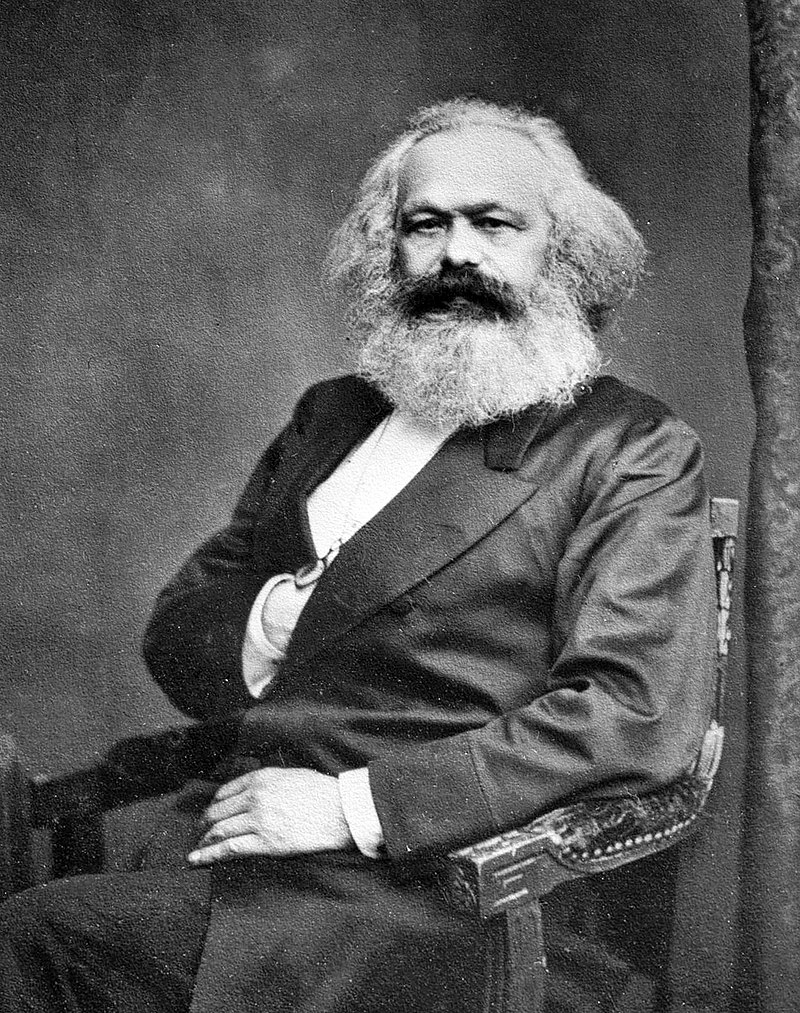
\includegraphics[width=0.3\textwidth]{800px-Karl_Marx_001}
    \caption{Karl Marx, 1875} \parencite{wiki:001}
\end{wrapfigure}
 
Curabitur ac augue sit amet enim pretium semper. Ut at finibus ligula. In hac habitasse platea dictumst. Duis porta felis lectus, non sollicitudin turpis ultricies in. Duis tristique justo feugiat elit sollicitudin, at efficitur sapien mollis. Etiam sem nisi, hendrerit vel bibendum non, vehicula vitae nibh. Aliquam commodo metus a dolor dignissim, sed lobortis nisl finibus. Fusce finibus, nibh et vehicula malesuada, diam massa semper ipsum, et volutpat lorem ipsum venenatis sapien. Quisque ac turpis tincidunt tortor vestibulum semper vel at magna. Nam erat nulla, egestas ac fringilla vehicula, tempor a velit.

Vestibulum ligula sem, dignissim eget consequat ac, volutpat eu erat. Sed sit amet iaculis leo, a pretium felis. Nunc justo erat, ullamcorper ut est et, tristique vulputate felis. Pellentesque habitant morbi tristique senectus et netus et malesuada fames ac turpis egestas. Donec gravida semper lacus eu sagittis. Donec tristique nec eros at tristique. Nulla interdum risus non metus lobortis vehicula. Sed ligula ante, pellentesque non nulla a, ullamcorper egestas ex. Nunc tincidunt rhoncus neque, ac luctus ligula interdum nec. Interdum et malesuada fames ac ante ipsum primis in faucibus.

\begin{wrapfigure}{l}{0.4\textwidth}
    \centering
    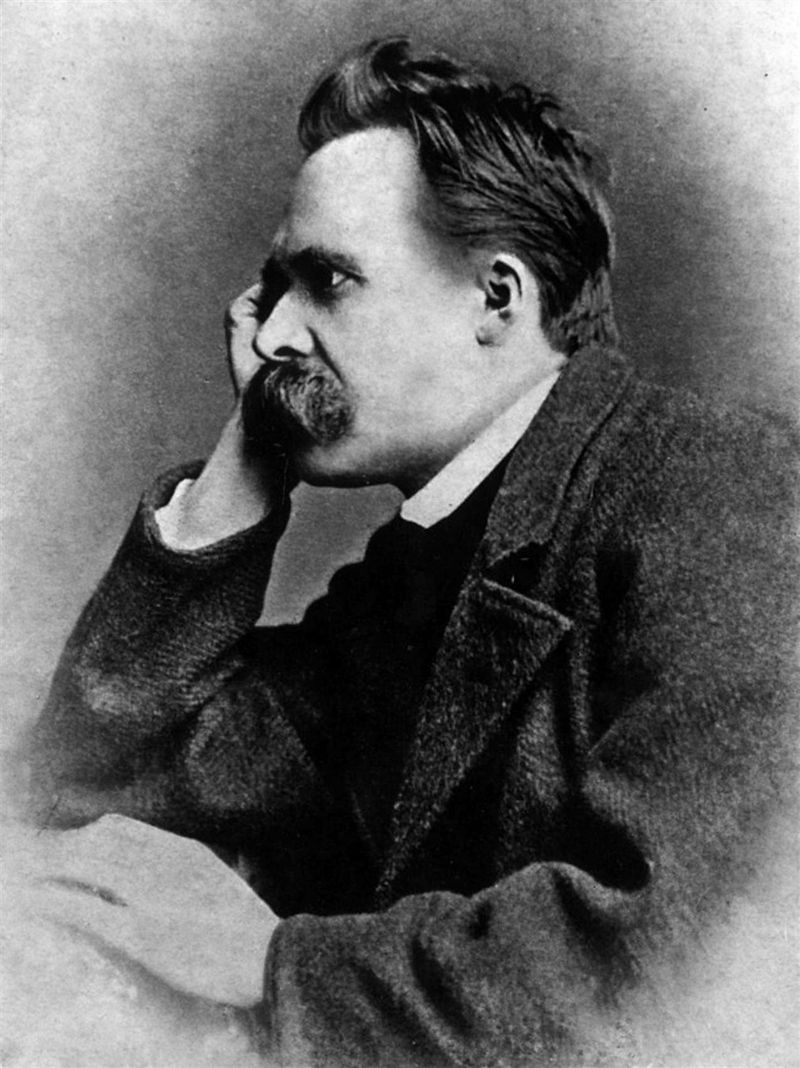
\includegraphics[width=0.4\textwidth]{800px-Nietzsche1882}
\caption{Friedrich Nietzsche, 1882} \parencite{wiki:002}
\end{wrapfigure}

Curabitur ac augue sit amet enim pretium semper. Ut at finibus ligula. In hac habitasse platea dictumst. Duis porta felis lectus, non sollicitudin turpis ultricies in. Duis tristique justo feugiat elit sollicitudin, at efficitur sapien mollis. Etiam sem nisi, hendrerit vel bibendum non, vehicula vitae nibh. Aliquam commodo metus a dolor dignissim, sed lobortis nisl finibus. Fusce finibus, nibh et vehicula malesuada, diam massa semper ipsum, et volutpat lorem ipsum venenatis sapien. Quisque ac turpis tincidunt tortor vestibulum semper vel at magna. Nam erat nulla, egestas ac fringilla vehicula, tempor a velit. Donec ipsum velit, porta nec iaculis ac, sollicitudin nec magna. Nullam pretium mauris et nulla fringilla, at vulputate tellus vulputate. Fusce venenatis nisi quis vestibulum facilisis. Suspendisse enim orci, blandit quis elementum ut, tincidunt id nisl.

Vestibulum ligula sem, dignissim eget consequat ac, volutpat eu erat. Sed sit amet iaculis leo, a pretium felis. Nunc justo erat, ullamcorper ut est et, tristique vulputate felis. Pellentesque habitant morbi tristique senectus et netus et malesuada fames ac turpis egestas. Donec gravida semper lacus eu sagittis. Donec tristique nec eros at tristique. Nulla interdum risus non metus lobortis vehicula. Sed ligula ante, pellentesque non nulla a, ullamcorper egestas ex. Nunc tincidunt rhoncus neque, ac luctus ligula interdum nec. Interdum et malesuada fames ac ante ipsum primis in faucibus.

Suspendisse faucibus libero sit amet varius scelerisque. Mauris eleifend ante quis libero pretium, efficitur eleifend est porttitor. Maecenas ac dictum sapien. Integer id dui vel augue luctus egestas non quis purus. Nam quis justo tempus, gravida lacus vitae, egestas magna. Proin ultrices quis tellus id ornare. Nulla ut pulvinar tellus. Mauris laoreet suscipit nisl, euismod vestibulum nisi. Proin vel mauris non sapien bibendum fringilla. Phasellus turpis arcu, viverra quis ultricies vel, ultricies in nunc. Integer quis arcu dictum, volutpat tortor vitae, iaculis risus. Vivamus leo enim, lobortis facilisis gravida nec, pulvinar nec metus. Etiam vulputate, velit eget ullamcorper lobortis, nibh urna porta quam, id placerat ipsum sem ac eros. In efficitur pulvinar orci, eget bibendum est porttitor sed. Maecenas tincidunt lacus tortor, eu dapibus est euismod at. Vestibulum sagittis tempus tincidunt. 

Lorem ipsum dolor sit amet, consectetur adipiscing elit. Nam rutrum magna ut mi sollicitudin pellentesque. Vivamus sit amet euismod nibh. Sed ornare enim vel tellus faucibus egestas. Donec sit amet diam placerat, interdum sapien sit amet, pulvinar neque. Morbi eget massa ut erat vehicula efficitur. Aenean vitae luctus magna. Nam varius ligula nec nunc egestas ultricies. Quisque vel vehicula mauris. Phasellus venenatis tortor et lorem aliquam luctus.

\section{Chapter 3, Section 2}

Curabitur ac augue sit amet enim pretium semper. Ut at finibus ligula. In hac habitasse platea dictumst. Duis porta felis lectus, non sollicitudin turpis ultricies in. Duis tristique justo feugiat elit sollicitudin, at efficitur sapien mollis. Etiam sem nisi, hendrerit vel bibendum non, vehicula vitae nibh. Aliquam commodo metus a dolor dignissim, sed lobortis nisl finibus. Fusce finibus, nibh et vehicula malesuada, diam massa semper ipsum, et volutpat lorem ipsum venenatis sapien. Quisque ac turpis tincidunt tortor vestibulum semper vel at magna. Nam erat nulla, egestas ac fringilla vehicula, tempor a velit. Donec ipsum velit, porta nec iaculis ac, sollicitudin nec magna. Nullam pretium mauris et nulla fringilla, at vulputate tellus vulputate. Fusce venenatis nisi quis vestibulum facilisis. Suspendisse enim orci, blandit quis elementum ut, tincidunt id nisl.

Vestibulum ligula sem, dignissim eget consequat ac, volutpat eu erat. Sed sit amet iaculis leo, a pretium felis. Nunc justo erat, ullamcorper ut est et, tristique vulputate felis. Pellentesque habitant morbi tristique senectus et netus et malesuada fames ac turpis egestas. Donec gravida semper lacus eu sagittis. Donec tristique nec eros at tristique. Nulla interdum risus non metus lobortis vehicula. Sed ligula ante, pellentesque non nulla a, ullamcorper egestas ex. Nunc tincidunt rhoncus neque, ac luctus ligula interdum nec. Interdum et malesuada fames ac ante ipsum primis in faucibus.

Suspendisse faucibus libero sit amet varius scelerisque. Mauris eleifend ante quis libero pretium, efficitur eleifend est porttitor. Maecenas ac dictum sapien. Integer id dui vel augue luctus egestas non quis purus. Nam quis justo tempus, gravida lacus vitae, egestas magna. Proin ultrices quis tellus id ornare. Nulla ut pulvinar tellus. Mauris laoreet suscipit nisl, euismod vestibulum nisi. Proin vel mauris non sapien bibendum fringilla. Phasellus turpis arcu, viverra quis ultricies vel, ultricies in nunc. Integer quis arcu dictum, volutpat tortor vitae, iaculis risus. Vivamus leo enim, lobortis facilisis gravida nec, pulvinar nec metus. Etiam vulputate, velit eget ullamcorper lobortis, nibh urna porta quam, id placerat ipsum sem ac eros. In efficitur pulvinar orci, eget bibendum est porttitor sed. Maecenas tincidunt lacus tortor, eu dapibus est euismod at. Vestibulum sagittis tempus tincidunt. 

Lorem ipsum dolor sit amet, consectetur adipiscing elit. Nam rutrum magna ut mi sollicitudin pellentesque. Vivamus sit amet euismod nibh. Sed ornare enim vel tellus faucibus egestas. Donec sit amet diam placerat, interdum sapien sit amet, pulvinar neque. Morbi eget massa ut erat vehicula efficitur. Aenean vitae luctus magna. Nam varius ligula nec nunc egestas ultricies. Quisque vel vehicula mauris. Phasellus venenatis tortor et lorem aliquam luctus. %% This loads the chapter03.tex file from the chapters sub directory. 
 
\chapter{Chapter 4 - Lists, Bullet Points and Columns}
%-------------------------------------------------
% CHAPTER 4
% This is a separate document for chapter 4 which is loaded into the main document.
%-------------------------------------------------

\section{Numbered Lists}

In this section I will demonstrate lists and bullet points. A numbered list is defined using the following code which is located between \verb|\begin{enumerate}| and \verb|\end{enumerate}|

\small

\begin{verbatim}
    \begin{enumerate}
    \item {This is item number 1}
    \item {This is item number 2}
    \item {This is item number 3}
    \end{enumerate}
\end{verbatim}

This code will look like this:

    \begin{enumerate}
    \item {This is item number 1}
    \item {This is item number 2}
    \item {This is item number 3}
    \end{enumerate}

We can also add other instructions, such as the colour of the text. The following code invokes the \verb|\textcolor{}{}| command. 

\begin{verbatim}
    \begin{enumerate}
    \item \textcolor{red}{This is an example of red text}
    \item \textcolor{black}{This is an example of black text}
    \item \textcolor{blue}{This is an example of blue text}
    \item \textcolor{green}{This is an example of green text}
    \end{enumerate}
\end{verbatim}
 
 This code will look like this:
 
    \begin{enumerate}
    \item \textcolor{red}{This is an example of red text}
    \item \textcolor{black}{This is an example of black text}
    \item \textcolor{blue}{This is an example of blue text}
    \item \textcolor{green}{This is an example of green text}
    \end{enumerate}

\normalsize

 This is how it will look if we have extended text:

    \begin{enumerate}
    \item {Quisque blandit nulla et velit auctor, a interdum ex imperdiet. Cras eget quam velit. Sed vel ante felis. Phasellus dictum lectus ac metus ornare facilisis. Aliquam placerat diam id viverra aliquam.}
    \item {Curabitur elit nulla, lacinia id euismod eu, elementum ullamcorper felis. Sed ut magna sit amet orci iaculis aliquet. Nulla facilisi. Sed elit nunc, posuere quis lorem a, vestibulum bibendum libero. }
    \item {Quisque blandit nulla et velit auctor, a interdum ex imperdiet. Cras eget quam velit.}
    \end{enumerate}

Quisque blandit nulla et velit auctor, a interdum ex imperdiet. Cras eget quam velit. Sed vel ante felis. Phasellus dictum lectus ac metus ornare facilisis. Aliquam placerat diam id viverra aliquam. Curabitur elit nulla, lacinia id euismod eu, elementum ullamcorper felis. Sed ut magna sit amet orci iaculis aliquet. Nulla facilisi. Sed elit nunc, posuere quis lorem a, vestibulum bibendum libero. Pellentesque ultricies est ut nisi finibus, ac commodo augue dictum. Vivamus laoreet sagittis placerat.

\newpage

\section{Bullet Points}

Bullet point done in a similar way to numbered lists, but instead of using the \verb|\begin{enumerate}| command we use \verb|\begin{itemize}| and \verb|\end{itemize}|

\begin{itemize}
\color{ForestGreen}
\item First item
\item Second item
\item Third item
\end{itemize}

Curabitur ac augue sit amet enim pretium semper. Ut at finibus ligula. In hac habitasse platea dictumst. Duis porta felis lectus, non sollicitudin turpis ultricies in. Duis tristique justo feugiat elit sollicitudin, at efficitur sapien mollis. Etiam sem nisi, hendrerit vel bibendum non, vehicula vitae nibh. Aliquam commodo metus a dolor dignissim, sed lobortis nisl finibus. Fusce finibus, nibh et vehicula malesuada, diam massa semper ipsum, et volutpat lorem ipsum venenatis sapien. Quisque ac turpis tincidunt tortor vestibulum semper vel at magna. Nam erat nulla, egestas ac fringilla vehicula, tempor a velit. Donec ipsum velit, porta nec iaculis ac, sollicitudin nec magna. Nullam pretium mauris et nulla fringilla, at vulputate tellus vulputate. Fusce venenatis nisi quis vestibulum facilisis. Suspendisse enim orci, blandit quis elementum ut, tincidunt id nisl.

Vestibulum ligula sem, dignissim eget consequat ac, volutpat eu erat. Sed sit amet iaculis leo, a pretium felis. Nunc justo erat, ullamcorper ut est et, tristique vulputate felis. Pellentesque habitant morbi tristique senectus et netus et malesuada fames ac turpis egestas. Donec gravida semper lacus eu sagittis. Donec tristique nec eros at tristique. Nulla interdum risus non metus lobortis vehicula. Sed ligula ante, pellentesque non nulla a, ullamcorper egestas ex. Nunc tincidunt rhoncus neque, ac luctus ligula interdum nec. Interdum et malesuada fames ac ante ipsum primis in faucibus.

\newpage

\begin{multicols}{2}
[
\section{Multiple Columns}
Suspendisse faucibus libero sit amet varius scelerisque. Mauris eleifend ante quis libero pretium, efficitur eleifend est porttitor. Maecenas ac dictum sapien. Integer id dui vel augue luctus egestas non quis purus.
]
Suspendisse faucibus libero sit amet varius scelerisque. Mauris eleifend ante quis libero pretium, efficitur eleifend est porttitor. Maecenas ac dictum sapien. Integer id dui vel augue luctus egestas non quis purus. Nam quis justo tempus, gravida lacus vitae, egestas magna. Proin ultrices quis tellus id ornare. Nulla ut pulvinar tellus. Mauris laoreet suscipit nisl, euismod vestibulum nisi. Proin vel mauris non sapien bibendum fringilla. Phasellus turpis arcu, viverra quis ultricies vel, ultricies in nunc. Integer quis arcu dictum, volutpat tortor vitae, iaculis risus. Vivamus leo enim, lobortis facilisis gravida nec, pulvinar nec metus. Etiam vulputate, velit eget ullamcorper lobortis, nibh urna porta quam, id placerat ipsum sem ac eros. In efficitur pulvinar orci, eget bibendum est porttitor sed. Maecenas tincidunt lacus tortor, eu dapibus est euismod at. Vestibulum sagittis tempus tincidunt. 

Lorem ipsum dolor sit amet, consectetur adipiscing elit. Nam rutrum magna ut mi sollicitudin pellentesque. Vivamus sit amet euismod nibh. Sed ornare enim vel tellus faucibus egestas. Donec sit amet diam placerat, interdum sapien sit amet, pulvinar neque. Morbi eget massa ut erat vehicula efficitur. Aenean vitae luctus magna. Nam varius ligula nec nunc egestas ultricies. Quisque vel vehicula mauris. Phasellus venenatis tortor et lorem aliquam luctus.

\end{multicols}

Suspendisse faucibus libero sit amet varius scelerisque. Mauris eleifend ante quis libero pretium, efficitur eleifend est porttitor. Maecenas ac dictum sapien. Integer id dui vel augue luctus egestas non quis purus. Nam quis justo tempus, gravida lacus vitae, egestas magna. Proin ultrices quis tellus id ornare. Nulla ut pulvinar tellus. Mauris laoreet suscipit nisl, euismod vestibulum nisi. Proin vel mauris non sapien bibendum fringilla. Phasellus turpis arcu, viverra quis ultricies vel, ultricies in nunc. Integer quis arcu dictum, volutpat tortor vitae, iaculis risus. Vivamus leo enim, lobortis facilisis gravida nec, pulvinar nec metus. Etiam vulputate, velit eget ullamcorper lobortis, nibh urna porta quam, id placerat ipsum sem ac eros. In efficitur pulvinar orci, eget bibendum est porttitor sed. Maecenas tincidunt lacus tortor, eu dapibus est euismod at. Vestibulum sagittis tempus tincidunt. 

Lorem ipsum dolor sit amet, consectetur adipiscing elit. Nam rutrum magna ut mi sollicitudin pellentesque. Vivamus sit amet euismod nibh. Sed ornare enim vel tellus faucibus egestas. Donec sit amet diam placerat, interdum sapien sit amet, pulvinar neque. Morbi eget massa ut erat vehicula efficitur. Aenean vitae luctus magna. Nam varius ligula nec nunc egestas ultricies. Quisque vel vehicula mauris. Phasellus venenatis tortor et lorem aliquam luctus.


\section{Lines}

Sometimes it necessary to place a horizonatl line between sections.

The \verb|\rule{6cm}{0.1pt}| command will print a horizontal line that is 6 centimetres long and 0.1 points thickness. In order for the horizontal line to print in the center of the page we have to enclose the \verb|\rule{6cm}{0.1pt}| command with \verb|\begin{center}| and \verb|\end{center}|

\begin{center}
    \rule{6cm}{0.1pt}
\end{center}

We can change it to this \verb|\rule{10cm}{3pt}| in order to print a horizontal line that is 10 centimetres long and 3 points thickness. 

\begin{center}
    \rule{10cm}{2pt}
\end{center}


A very nice option to break sections is instruct LaTeX to print a dotted line. This is done with the  can change it to this \verb|\dotfill| command and looks like this. 

 \dotfill

Lorem ipsum dolor sit amet, consectetur adipiscing elit. Nam rutrum magna ut mi sollicitudin pellentesque. Vivamus sit amet euismod nibh. Sed ornare enim vel tellus faucibus egestas. Donec sit amet diam placerat, interdum sapien sit amet, pulvinar neque. Morbi eget massa ut erat vehicula efficitur. Aenean vitae luctus magna. Nam varius ligula nec nunc egestas ultricies. Quisque vel vehicula mauris. Phasellus venenatis tortor et lorem aliquam luctus.
 %% This loads the chapter04.tex file from the chapters sub directory. 
 
\chapter{Conclusion}


Lorem ipsum dolor sit amet, consectetur adipiscing elit. Nam rutrum magna ut mi sollicitudin pellentesque. Vivamus sit amet euismod nibh. Sed ornare enim vel tellus faucibus egestas. Donec sit amet diam placerat, interdum sapien sit amet, pulvinar neque. Morbi eget massa ut erat vehicula efficitur. Aenean vitae luctus magna. Nam varius ligula nec nunc egestas ultricies. Quisque vel vehicula mauris. Phasellus venenatis tortor et lorem aliquam luctus.

Quisque blandit nulla et velit auctor, a interdum ex imperdiet. Cras eget quam velit. Sed vel ante felis. Phasellus dictum lectus ac metus ornare facilisis. Aliquam placerat diam id viverra aliquam. Curabitur elit nulla, lacinia id euismod eu, elementum ullamcorper felis. Sed ut magna sit amet orci iaculis aliquet. Nulla facilisi. Sed elit nunc, posuere quis lorem a, vestibulum bibendum libero. Pellentesque ultricies est ut nisi finibus, ac commodo augue dictum. Vivamus laoreet sagittis placerat.

Curabitur ac augue sit amet enim pretium semper. Ut at finibus ligula. In hac habitasse platea dictumst. Duis porta felis lectus, non sollicitudin turpis ultricies in. Duis tristique justo feugiat elit sollicitudin, at efficitur sapien mollis. Etiam sem nisi, hendrerit vel bibendum non, vehicula vitae nibh. Aliquam commodo metus a dolor dignissim, sed lobortis nisl finibus. Fusce finibus, nibh et vehicula malesuada, diam massa semper ipsum, et volutpat lorem ipsum venenatis sapien. Quisque ac turpis tincidunt tortor vestibulum semper vel at magna. Nam erat nulla, egestas ac fringilla vehicula, tempor a velit. Donec ipsum velit, porta nec iaculis ac, sollicitudin nec magna. Nullam pretium mauris et nulla fringilla, at vulputate tellus vulputate. Fusce venenatis nisi quis vestibulum facilisis. Suspendisse enim orci, blandit quis elementum ut, tincidunt id nisl.

Vestibulum ligula sem, dignissim eget consequat ac, volutpat eu erat. Sed sit amet iaculis leo, a pretium felis. Nunc justo erat, ullamcorper ut est et, tristique vulputate felis. Pellentesque habitant morbi tristique senectus et netus et malesuada fames ac turpis egestas. Donec gravida semper lacus eu sagittis. Donec tristique nec eros at tristique. Nulla interdum risus non metus lobortis vehicula. Sed ligula ante, pellentesque non nulla a, ullamcorper egestas ex. Nunc tincidunt rhoncus neque, ac luctus ligula interdum nec. Interdum et malesuada fames ac ante ipsum primis in faucibus.

Suspendisse faucibus libero sit amet varius scelerisque. Mauris eleifend ante quis libero pretium, efficitur eleifend est porttitor. Maecenas ac dictum sapien. Integer id dui vel augue luctus egestas non quis purus. Nam quis justo tempus, gravida lacus vitae, egestas magna. Proin ultrices quis tellus id ornare. Nulla ut pulvinar tellus. Mauris laoreet suscipit nisl, euismod vestibulum nisi. Proin vel mauris non sapien bibendum fringilla. Phasellus turpis arcu, viverra quis ultricies vel, ultricies in nunc. Integer quis arcu dictum, volutpat tortor vitae, iaculis risus. Vivamus leo enim, lobortis facilisis gravida nec, pulvinar nec metus. Etiam vulputate, velit eget ullamcorper lobortis, nibh urna porta quam, id placerat ipsum sem ac eros. In efficitur pulvinar orci, eget bibendum est porttitor sed. Maecenas tincidunt lacus tortor, eu dapibus est euismod at. Vestibulum sagittis tempus tincidunt.  %% This loads the conclusion.tex file from the chapters sub directory. 

%---------------------------------------------------------- 
% APPENDIX
% This is the Appendix section 
%----------------------------------------------------------

%% To add an appendix at the end of the document we we use the \appendix command. Following the same structure as the chapters the appendix.tex file will be kept in the chapters folder.  

\appendix %% This tells LaTeX that what follows is an appendix. After this command chapters will be numbered with letters. 

\chapter{Appendix}

\input{chapters/appendix}

%---------------------------------------------------------- 
% REFERENCES
% This is the references section 
%----------------------------------------------------------

\backmatter %% should be inserted before the very last items in the document,such as the bibliography and the index.  In the standard document classes, this has no visual effect.

\setlength{\bibitemsep}{1.6\itemsep} %% This command sets the space between the bibliography entries. 

\nocite{*} %% The \nocite{*} command can be used to if we want to reference all entries in the references.bib file. This is useful because we might want to include material that is not directly referenced. 


\printbibliography[heading=bibintoc,title={References}] %% This command prints the bibliography. The parameter heading=bibintoc prints the bibliography in the Table of Contents. We can use the parameter title={} to specify the bibliography title if we do no want the default Bibliography.  


\end{document}
